% !TEX program = pdflatex
% Springer LNCS proceedings format (llncs.cls + splncs04.bst in this folder).
\documentclass[runningheads]{llncs}
%
\usepackage[T1]{fontenc}
\usepackage{graphicx}
\graphicspath{{Figures/}{../Figures/}}
\usepackage{booktabs}
\usepackage{amsmath}
\usepackage{amssymb}

\sloppy

\begin{document}

\title{Visual Attention is Not Memoryless: Higher-Order Sequence Modeling of TeamLead Gaze in VR Cardiac Arrest Simulation}

\titlerunning{Higher-Order Gaze Modeling in VR}

% Uncomment for camera-ready submission; comment out for blind review.
\author{Haoting Gao\inst{1}\orcidID{0009-0002-8159-1975}\thanks{Corresponding author.} \and
Kapotaksha Das\inst{1,2}\orcidID{0000-0001-9920-4668} \and Liang Zhang\inst{1}\orcidID{0009-0002-0017-2569} \and
Mohamed Abouelenien\inst{2}\orcidID{0000-0001-5351-5778} \and
Michael Cole\inst{3}\orcidID{0009-0000-4146-3632} \and
James Cooke\inst{1}\orcidID{0000-0002-4761-7185} \and
Vitaliy Popov\inst{1}\orcidID{0000-0003-2348-5285}}

\authorrunning{Gao et al.}

\institute{Department of Learning Health Sciences, University of Michigan Medical School, Ann Arbor, MI, USA\\
\email{haotin@umich.edu, cookej@umich.edu, vipopov@umich.edu} \and
Computer and Information Sciences, University of Michigan-Dearborn, Dearborn, MI, USA\\
\email{takposha@umich.edu, zmohamed@umich.edu} \and
Department of Emergency Medicine, University of Michigan Medical School, Ann Arbor, MI, USA\\
\email{mcolemd@umich.edu}}

\maketitle

\begin{abstract}
  Caring for critically ill patients requires healthcare professionals to make cognitively demanding decisions under severe time and information constraints. Simulation-based training has proven a successful strategy to prepare clinicians for such low-frequency, high-risk events in a safe setting. Clinical simulation also makes this a perfect setting to study how team leaders structure their visual attention during these scenarios by continuously shifting gaze among the patient, vital-sign monitors, resuscitation equipment, and teammates to build situational awareness. In this paper, we examine these gaze transitions by mapping each fixation to one of seven clinically defined areas of interest (AOIs), such as the patient, vitals monitor, or resuscitation equipment, and modeling sequences of AOI changes. First-order Markov models, commonly used in gaze analysis, treat this process as memoryless, i.e., the next AOI is assumed to depend only on the current AOI. This assumption may overlook structured gaze cycles (i.e., brief, recurrent sequences) that reflect deliberate monitoring rather than e.g., searching or overfixation behavior. Capturing such cycles may be essential to accurately characterizing how team leads actively track and integrate clinical information during patient care. We analyze TeamLead AOI sequences from $n{=}14$ simulation sessions (one TeamLead sequence per session), using $k$-th-order Markov models with Laplace smoothing and leave-one-session-out cross-validation. Our results show that, among candidate orders $k \in \{1,2,3,4,5\}$, a second-order model ($k{=}2$) maximizes held-out mean log-likelihood and outperforms the first-order baseline on all three metrics (mean $\Delta$ log-likelihood $+0.086$, accuracy $+0.11$, macro-F$_1$ $+0.14$; all $p<0.001$). A model that also accounted for scenario stage outperformed the first-order baseline but performed worse than the AOI-only second-order model. Thus, in this sample, scenario stage provided little additional predictive information beyond the two most recent AOIs. The second-order model’s improvement was driven primarily by short return-to-anchor patterns (e.g., monitor → patient → monitor), consistent with team leaders repeatedly revisiting key information sources during patient monitoring.

\keywords{higher-order Markov model \and gaze analysis \and situational awareness \and virtual reality simulation \and cardiac arrest training}
\end{abstract}

\section{Introduction}

In high-stakes, time-critical clinical environments, situational awareness (SA) is essential for effective team performance~\cite{popov2025communication}. Cardiac arrest is a prototypical example of such an environment, where patient status can deteriorate within minutes, and care team members must rapidly recognize rhythm changes, coordinate role-specific actions, and execute time-critical therapeutic interventions~\cite{nallamothu2018resuscitation}. These demands are not distributed evenly across team members. The TeamLead, in particular, must monitor task progress, coordinate team activity~\cite{kolbe2013co}, and reallocate attention as clinical demands evolve~\cite{gao2026towards}. Because visual attention provides an observable trace of Level~1 SA (perception of environmental cues)~\cite{ensley1995toward}, gaze data have become a valuable proxy for studying how SA is maintained during team-based clinical work~\cite{caloca2024exploring,weinberg2020visual}. However, SA in acute care settings is not static. TeamLeads must continuously update their understanding of patient status, team actions, and scenario progress as events unfold over time. This dynamic nature makes the temporal organization of gaze especially important, because where the TeamLead looks next may depend not only on the current clinical cue but also on the recent sequence of attended information.

To examine whether TeamLead gaze exhibits such history-dependent temporal structure, we apply higher-order network (HON) analysis to TeamLead AOI sequences in multi-person virtual reality (VR) cardiac arrest simulation. HON extends first-order transition modeling by representing cases in which the next state depends on recent path history in addition to the current state~\cite{xuRepresentingHigherorderDependencies2016}, making it well suited for detecting short recurring patterns between AOIs. We situate the analysis in VR-based simulation, where SA and teamwork are central to performance and where immersive, standardized scenarios enable consistent behavioral trace data collection~\cite{rosen2015integrative}. We compare a first-order Markov baseline with HON under leave-one-session-out cross-validation, and test whether adding explicit annotated clinical-stage context improves prediction. Specifically, we ask two research questions:
\begin{itemize}
  \item[\textbf{RQ1.}] Does higher-order modeling improve next-AOI prediction beyond a first-order baseline in TeamLead AOI sequences?
  \item[\textbf{RQ2.}] To what extent does adding clinical-stage context affect the predictive value of higher-order AOI sequence modeling?
\end{itemize}

We frame this study as a foundational proof-of-concept study based on a single scenario, and our analysis draws on 14 TeamLead simulation sessions.

\section{Related Work}

\textbf{Gaze and situational awareness in clinical simulation.}
Endsley's three-level model frames SA as the perception of cues, the comprehension of their meaning, and the projection of future state~\cite{ensley1995toward}. Because gaze provides an observable trace of Level~1 perception, eye-tracking has become a widely used proxy for SA in time-critical clinical settings~\cite{caloca2024exploring,weinberg2020visual}, where studies link aggregate gaze metrics (fixation counts, dwell times, AOI proportions) to leader behaviors and team performance, and multimodal extensions combine gaze with pose or speech to characterize teamwork during training~\cite{rosen2015integrative,popov2025communication}. These studies typically describe \emph{where} attention is allocated but do not directly test the sequential generative process underlying those allocations.

\textbf{Transition- and network-based analyses of gaze.}
A second body of work models visual attention as transitions between AOIs. Gaze transition entropy quantifies how unpredictable next-fixation behavior is given the current AOI~\cite{krejtz2015gaze}, and Transition Network Analysis (TNA) has been proposed as a general framework for modeling transition structure in learning analytics data~\cite{saqr2025transition}; prior work applied first-order TNA to multi-role gaze in a multiperson VR resuscitation dataset to characterize role- and stage-specific differences in attentional structure~\cite{gao2026towards}, and related ordered-network approaches extend the idea to team communication~\cite{popov2025communication}. Critically, transitions are estimated from \emph{first-order} statistics, treating the next AOI as dependent on the current AOI alone. Such quantities cannot, by construction, distinguish two visits to the same AOI that originate from different short histories. In this study, we test whether that assumption is empirically warranted for TeamLead visual attention, using held-out predictive performance.

\textbf{Higher-order models for path-dependent behavior.}
Path-dependent processes that violate the first-order assumption have been studied extensively. Xu et al.~\cite{xuRepresentingHigherorderDependencies2016} introduce higher-order networks (HON) as a representation that selectively retains longer-history contexts when those contexts carry additional predictive power, and Scholtes~\cite{scholtesWhenNetworkNetwork2017} formalizes the choice of order $k$ as a multi-order model-selection problem. Two observations motivate our choices. First, higher-order gains typically concentrate in a few ``surprising'' contexts 
## define why use surprising contexts> what does it refer to?
where future state genuinely depends on more than the current node~\cite{xuRepresentingHigherorderDependencies2016,scholtesWhenNetworkNetwork2017}, a pattern well suited to supervisory monitoring routines. Second, with a small alphabet (seven AOIs) and a modest corpus, fixed-order Markov models with smoothing are a simple, interpretable instantiation of higher-order modeling. Our contribution is an empirical test of utilizing HON modeling in visual attention prediction (## define what specifically about this extension) yields predictive benefits on TeamLead gaze beyond first-order analyses, and a characterization of \emph{which} patterns explain clinically meaningful behaviors.

\section{Methods}
\textbf{Data and Areas of Interest.} Eye-tracking data captured from a multi-person VR cardiac arrest simulations in which teams of four trainees managed scenarios in standardized roles (TeamLead, Airway, CPR, Defib) following American Heart Association guidelines~\cite{perman20242023}. During resuscitation, Airway, CPR, and Defib providers focus on role-specific interventions (e.g., ventilation, compressions, and defibrillation), whereas the TeamLead coordinates the team, monitors patient status and overall task progress, and directs time-critical treatment decisions~\cite{nallamothu2018resuscitation,kolbe2013co}. We therefore analyze TeamLead gaze as the supervisory attention stream most likely to integrate information across the patient, monitor, equipment, and teammates. Gaze was recorded with HP Reverb G2 Omnicept headsets using the Cognitive3D platform~\cite{Cognitive3D}; the AOI scheme and preprocessing pipeline follow those documented for this dataset~\cite{gao2026towards}. The scenario follows a STEMI cardiac arrest~\cite{thygesen2018fourth} that progresses from ventricular tachycardia with a weak pulse through pulseless VT, asystole, and ventricular fibrillation before return of circulation. Data collection was approved by the Institutional Review Board (IRB protocol HUM00193383). We analyzed the \textbf{14} sessions that provided complete, continuous TeamLead eye-tracking coverage together with clinical-stage annotation, one TeamLead sequence per session; recordings with interrupted tracking or missing stage annotations were excluded. Sessions averaged 13.1~min (SD~=~3.6). The TeamLead role produced 31{,}157 raw fixations; after discarding fixations without a valid AOI and collapsing consecutive fixations on the same AOI, 8{,}798 AOI dwell events and 8{,}784 AOI transitions remained across the 14 sessions and served as the input to all sequence models.

Gaze was mapped to seven AOIs (Table~\ref{tab:AOIs}): airway, CPR, defibrillation, and medication/IV equipment; the patient vitals monitor; the patient; and other team members.

\begin{table}[t]
\centering
\caption{Areas of Interest (AOIs) used for gaze-sequence analysis.}
\label{tab:AOIs}
\begin{tabular}{ll}
\toprule
\textbf{AOI} & \textbf{Description} \\
\midrule
Equipment - Airway     & Airway management equipment (e.g., bag-valve masks). \\
Equipment - CPR        & Hands and UI (user interface) elements directly involved in CPR. \\
Equipment - Defib      & Defibrillator unit and associated controls. \\
Equipment - Meds \& IV & Medication- and IV-related objects. \\
Patient Vitals Monitor & ECG, SpO2, respiration, and related vitals. \\
Other Team Members     & 3D avatars of other people in session. \\
Patient                & Virtual patient body. \\
\bottomrule
\end{tabular}
\end{table}

\textbf{AOI Sequences and Higher-Order Markov Modeling.} To examine whether TeamLead gaze follows a memoryless process or a history-dependent sequence process, we modeled each TeamLead's gaze behavior as a time-ordered sequence of seven clinically meaningful AOIs. This framing treats each fixation as an observation of where the TeamLead allocated visual attention and asks whether the next AOI can be predicted from the immediately preceding AOI alone, as assumed by a first-order Markov model, or whether prediction improves when recent AOI history is included. 

Each valid fixation was mapped to a single AOI label and ordered by timestamp to form a role-specific AOI sequence; fixations without valid labels and saccade samples were excluded. Consecutive repeated labels were collapsed so that each step corresponds to a change of AOI (a transition event), and fixations landing on a non-clinical region outside the seven AOIs (an artifact of VR locomotion, e.g., teleport-based navigation) were removed before collapsing. Analyses focus on the \textbf{TeamLead} sequence for each session.

Let $(x_1,\ldots,x_T)$ denote a TeamLead AOI sequence over the seven labels. For a fixed context length $k \geq 1$, each prediction position $t \in \{k+1,\ldots,T\}$ uses context $\mathbf{c}_t = (x_{t-k},\ldots,x_{t-1})$ and outcome $x_t$. Counts $N(\mathbf{c}, a)$ accumulate how often label $a$ follows context $\mathbf{c}$ in training. Because higher-order contexts can be sparse, especially when evaluating held-out sessions, transition probabilities were estimated with additive (Laplace) smoothing~\cite{chen1999empirical} using $\alpha = 0.5$ over the closed vocabulary of seven AOIs. This assigns a small amount of probability mass to unseen but possible transitions and prevents zero probabilities from dominating the held-out log-likelihood:
\[
\widehat{P}(x_t = a \mid \mathbf{c}_t) = \frac{N(\mathbf{c}_t, a) + \alpha}{\sum_{a'} N(\mathbf{c}_t, a') + 7\alpha}.
\]
When $k=1$, the model reduces to a standard first-order Markov chain in which the next AOI depends only on the current AOI. When $k>1$, each distinct length-$k$ history defines a higher-order context, allowing the predicted next AOI to depend on recent sequence history. Throughout, we refer to this smoothed fixed-order model as our higher-order network (HON) instantiation: it captures history dependence through explicit length-$k$ contexts rather than the pruned, rule-based HON graph of Xu et al.~\cite{xuRepresentingHigherorderDependencies2016}. The \emph{predicted} next AOI is the argmax under $\widehat{P}(\cdot \mid \mathbf{c}_t)$. Session-level \textbf{mean log-likelihood} averages $\log \widehat{P}(x_t \mid \mathbf{c}_t)$ over scored transitions; \textbf{accuracy} is the fraction of correct argmax predictions; \textbf{macro-F$_1$} averages per-class F$_1$ over the seven AOIs. We report these three metrics because they are complementary: mean log-likelihood is a proper scoring rule~\cite{gneiting2007strictly} sensitive to the full predicted distribution and serves as our model-selection criterion; accuracy summarizes hard next-AOI prediction but is dominated by frequent AOIs; and macro-F$_1$ weights all seven AOIs equally, revealing whether history helps recover less frequent destinations.

\textbf{Evaluation and order selection.} Models were fit under \textbf{leave-one-session-out (LOSO)} cross-validation: for each of 14 sessions, parameters were estimated from all other sessions and evaluated on the held-out TeamLead sequence, avoiding within-session leakage. Order $k$ was selected from $\{1,2,3,4,5\}$ by maximizing the mean held-out log-likelihood across folds. Bayesian Information Criterion (BIC)~\cite{schwarz1978estimating} summaries on training folds were retained for reference but were not the primary rule, as BIC favored $k{=}1$ despite stronger held-out likelihood for larger $k$.

To test whether clinical stage improves prediction beyond AOI history, we fit a stage-conditioned model. Clinical stages were annotated from the scenario's scripted cardiac rhythm timeline, which assigns each rhythm phase (e.g., ventricular tachycardia, asystole, ventricular fibrillation, and return of spontaneous circulation) start and end timestamps; because different rhythms prioritize different information (e.g., defibrillator and monitor during shockable rhythms versus patient and airway during compressions), the cardiac arrest stage could in principle inform next-AOI prediction. The model estimates separate $k$-th-order count tables for each stage while sharing the same order $k$. At each prediction position $t$, the model conditions on the clinical stage annotated at that time index. Sparse $(\text{stage}, \mathbf{c}_t)$ combinations use hierarchical back-off: stage-specific counts when available, otherwise the global $k$-th-order model, then the global first-order model, then a uniform distribution.

For each session and metric, we computed paired differences between the higher-order model at the selected $k$ and the first-order baseline ($k{=}1$) on the same held-out sequence. Because sessions were not assumed to follow a normal distribution, we tested whether median paired differences differed from zero using the \textbf{Wilcoxon signed-rank} test on the 14 session-level deltas.

We also summarized recurring higher-order sequences induced by the fitted model. For each observed length-$k$ context with sufficient support, we recorded the most probable next AOI and its empirical support. When $k{=}2$, such contexts correspond to weighted AOI triplets $x_{t-2}{\rightarrow}x_{t-1}{\rightarrow}x_t$ that highlight short return-to-anchor routines invisible to a memoryless model; they are used descriptively in Section~\ref{sec:results} to interpret \emph{where} the model gains information.

\section{Results \& Discussion}
\label{sec:results}

We compared two higher-order specifications, both using the selected order $k{=}2$: an \emph{AOI-only} model that conditions on AOI history alone, and a \emph{stage-conditioned} model that additionally splits transition counts by clinical stage. We organize the results around the two research questions: Section~\ref{sec:order_selection} establishes the optimal order; Section~\ref{sec:stageA} addresses RQ1 with the AOI-only model; Section~\ref{sec:stageB} addresses RQ2 by adding stage conditioning; Section~\ref{sec:motifs} interprets which contexts drive the gain.

\subsection[Order selection]{Order selection: $k{=}2$ is optimal}\label{sec:order_selection}

\begin{figure}[t]
\centering
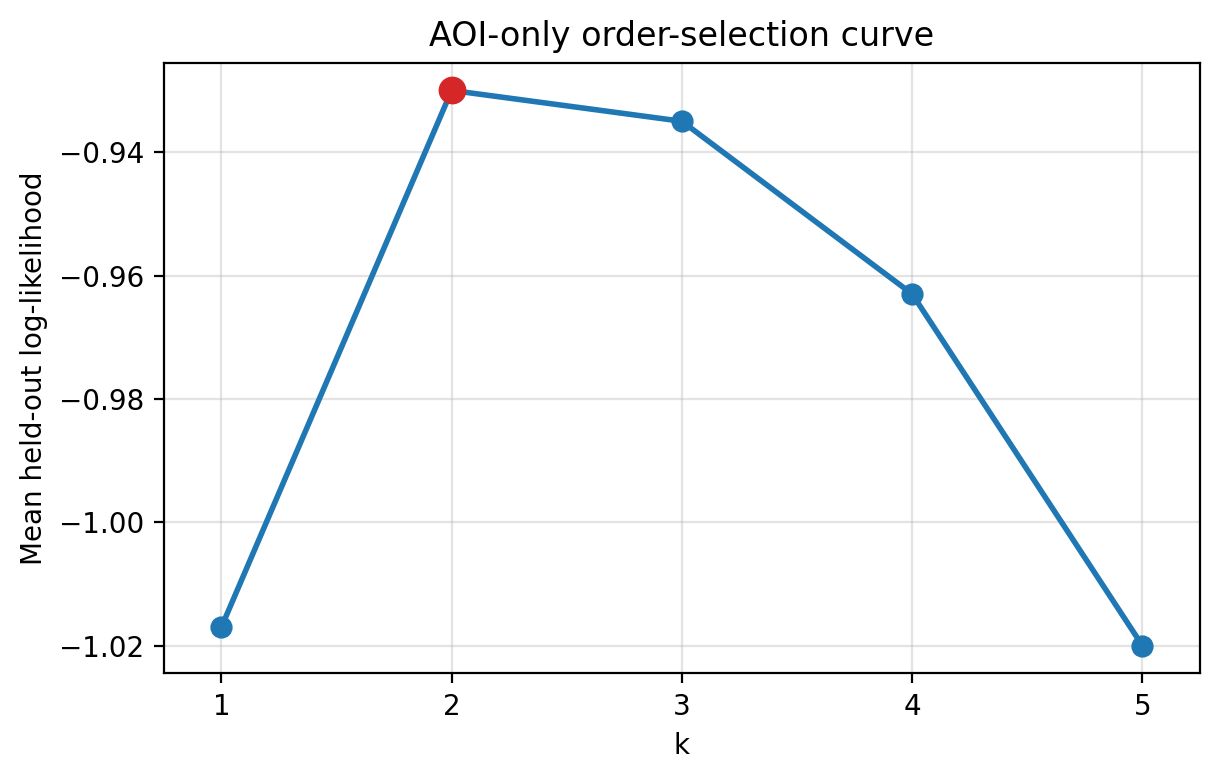
\includegraphics[width=0.75\textwidth]{aoi_stageA_all_k_curve.png}
\caption{Order-selection curve for the AOI-only model: mean held-out log-likelihood across LOSO folds vs.\ Markov order $k$. Performance peaks at $k{=}2$ and degrades for $k \geq 3$ as context tables fragment.}
\label{fig:k_curve}
\vspace{-6pt}
\end{figure}

Held-out mean log-likelihood as a function of $k$ (Fig.~\ref{fig:k_curve}) is non-monotone: a sharp gain from $k{=}1$ ($\approx -1.017$) to $k{=}2$ ($\approx -0.930$), followed by steady decline for $k{=}3,4,5$ as the number of distinct length-$k$ contexts grows and per-context counts become sparse on a 7-AOI alphabet with 14 sessions. The relevant memory in TeamLead AOI sequences is therefore short: most predictable structure is captured by conditioning on the previous \emph{two} fixations. We used $k{=}2$ for all subsequent comparisons, consistent with HON practice favoring compact, well-supported contexts~\cite{xuRepresentingHigherorderDependencies2016}.

\subsection[RQ1: higher-order gain]{Higher-order modeling improves next-AOI prediction (RQ1)}\label{sec:stageA}

\begin{figure}[t]
\centering
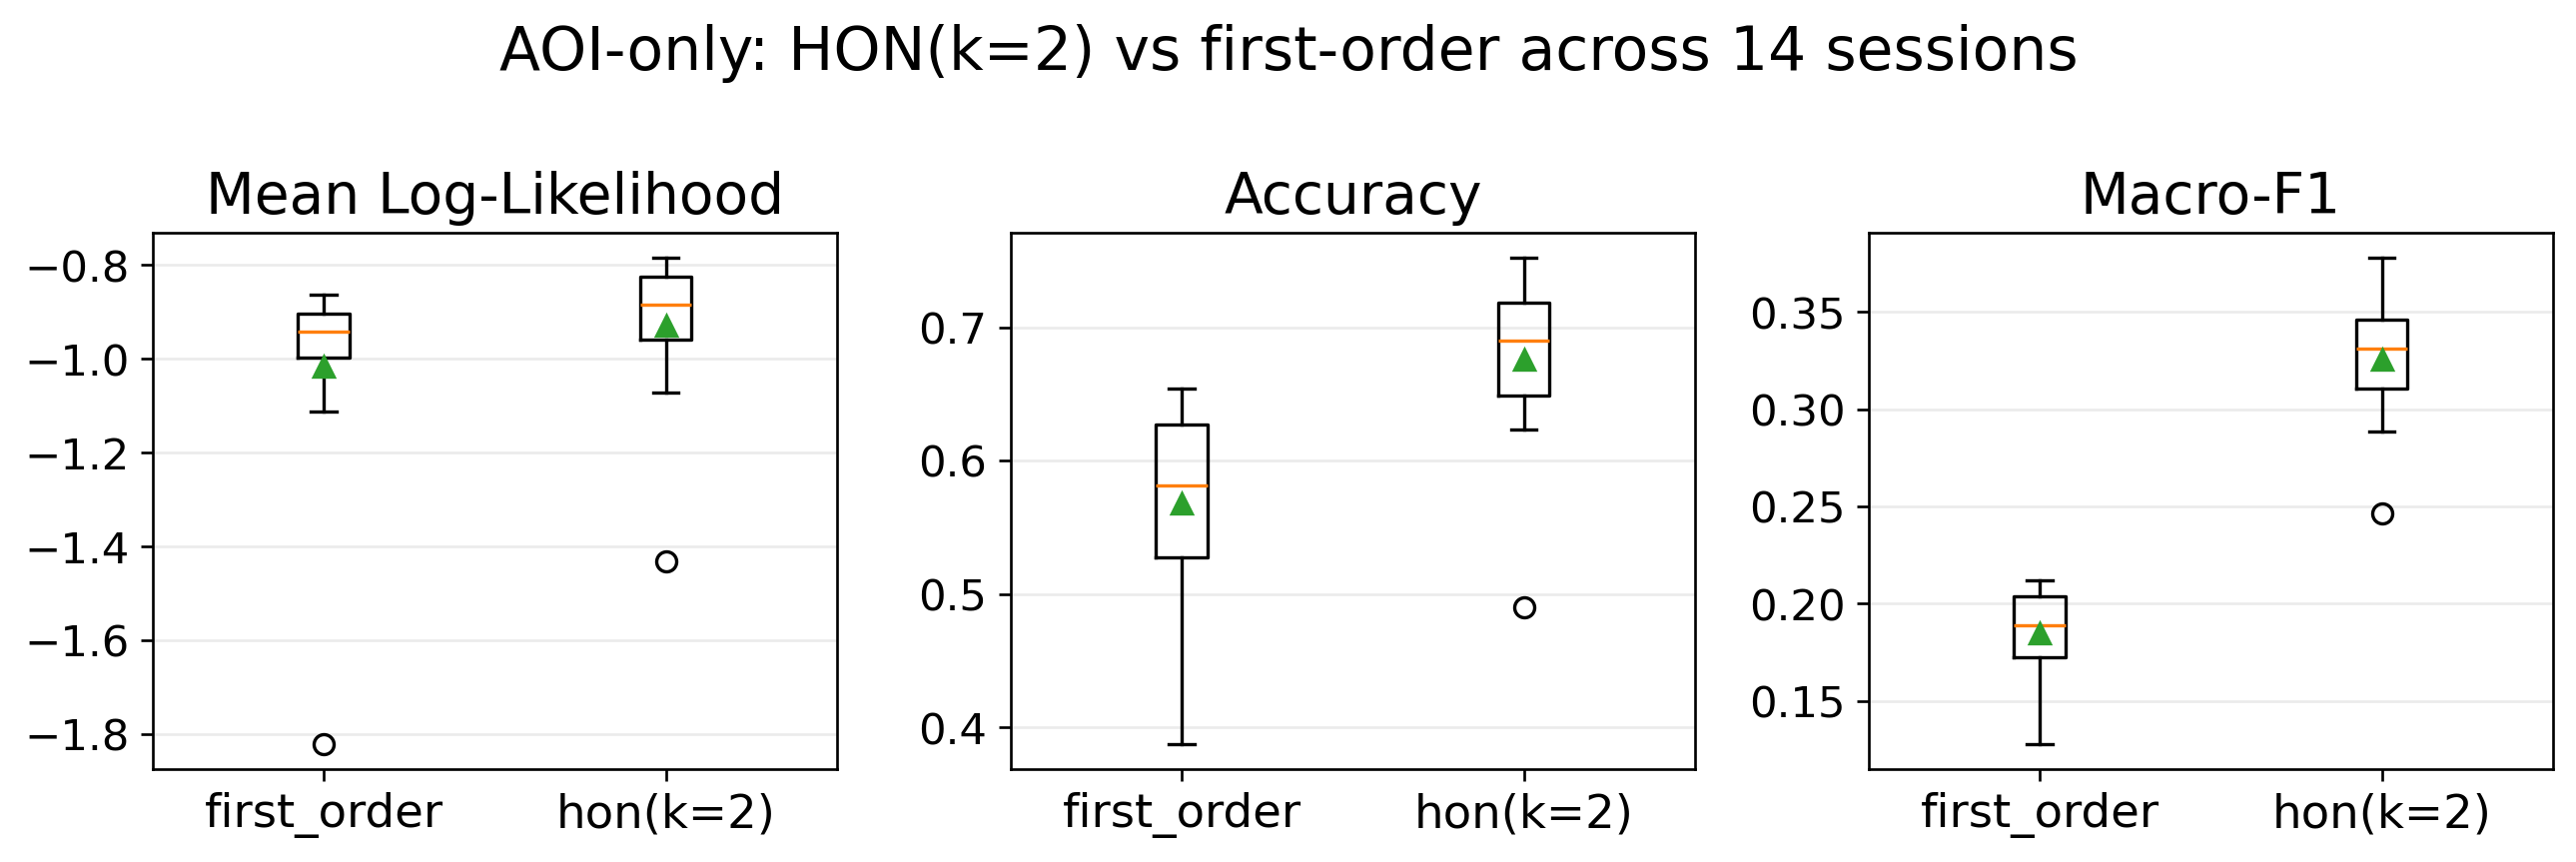
\includegraphics[width=1\textwidth]{stageA_vs_firstorder_metrics.png}
\caption{AOI-only HON($k{=}2$) versus first-order baseline across 14 LOSO folds on three session-level metrics. Boxes show medians and IQR; triangles mark means. HON improves all three metrics on the majority of sessions.}
\label{fig:stageA_metrics}
\vspace{-6pt}
\end{figure}

\begin{table}[t]
\centering
\caption{AOI-only model: paired session-level deltas (HON($k{=}2$) $-$ first-order) across 14 LOSO folds, two-sided Wilcoxon signed-rank tests.}
\label{tab:stageA}
\begin{tabular}{lccc}
\toprule
\textbf{Metric} & \textbf{Mean $\Delta$} & \textbf{Wilcoxon $p$} & \textbf{Direction} \\
\midrule
Mean log-likelihood & $+0.0858$ & $0.00037$ & HON $>$ first-order \\
Accuracy            & $+0.1081$ & $0.00012$ & HON $>$ first-order \\
Macro-F$_1$         & $+0.1411$ & $0.00012$ & HON $>$ first-order \\
\bottomrule
\end{tabular}
\end{table}

In the AOI-only model, HON($k{=}2$) outperforms the first-order baseline on all three metrics (Fig.~\ref{fig:stageA_metrics}; Table~\ref{tab:stageA}). Mean log-likelihood improves by $+0.0858$ nats (natural-log units) per scored transition ($p = 0.00037$), a multiplicative likelihood gain of roughly $9\%$ per step. Argmax accuracy improves from a median around $0.58$ to $0.69$ ($\Delta = +0.108$, $p = 0.00012$), and macro-F$_1$---which weights minority AOIs equally---increases by roughly three-quarters, from $\approx 0.19$ to $\approx 0.33$ ($\Delta = +0.141$, $p = 0.00012$). The macro-F$_1$ gain is informative: HON does not merely sharpen predictions for the most frequent AOIs (e.g., \textit{Patient Vitals Monitor}) but recovers structure around less frequent destinations whose distribution depends on which AOI the TeamLead just came from. This answers RQ1: the first-order assumption underlying transition-based gaze analyses~\cite{krejtz2015gaze,saqr2025transition,gao2026towards} is empirically too restrictive for TeamLead gaze, and a compact $k{=}2$ history yields a reliable, substantial improvement. Bootstrap $95\%$ confidence intervals over the 14 folds exclude zero for all three metrics (log-likelihood $[+0.05,+0.14]$, accuracy $[+0.09,+0.13]$, macro-F$_1$ $[+0.13,+0.15]$), so the gain does not rest on a few sessions. Practically, correctly anticipating these less frequent, history-dependent transitions---not only the dominant monitor fixation---is what an attention-aware debriefing or feedback tool would require to flag atypical monitoring, which motivates the clinical directions discussed below.

\subsection[RQ2: stage context]{Adding clinical-stage context does not help (RQ2)}\label{sec:stageB}

\begin{figure}[t]
\centering
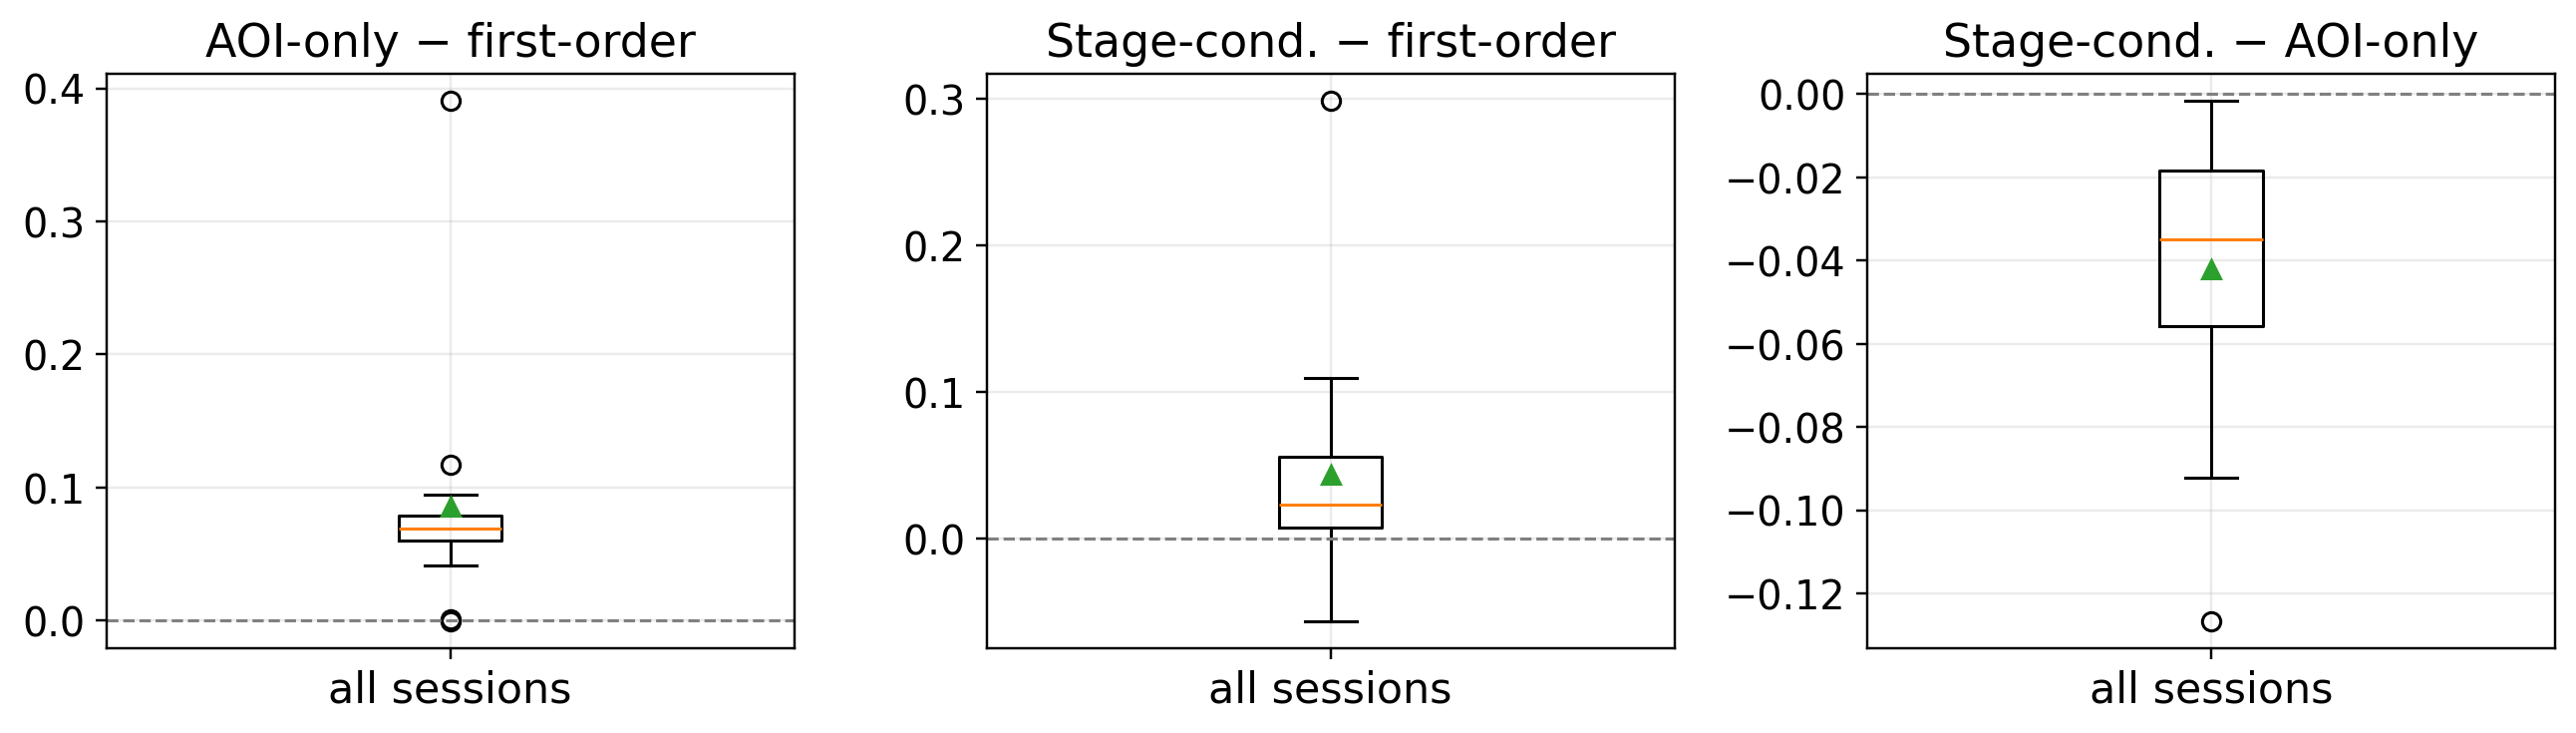
\includegraphics[width=1\textwidth]{aoi_stageA_stageB_ll_deltas.png}
\caption{Per-session log-likelihood deltas. \textbf{Left:} AOI-only HON($k{=}2$) $-$ first-order, mean $+0.0858$ ($p{=}0.00037$). \textbf{Middle:} stage-conditioned $-$ first-order, mean $+0.0437$ ($p{=}0.0166$). \textbf{Right:} context effect, stage-conditioned $-$ AOI-only, mean $-0.0421$ ($p{=}0.00012$). Stage-conditioning beats first-order but is dominated by the AOI-only model.}
\label{fig:context_effect}
\vspace{-6pt}
\end{figure}

The stage-conditioned model also outperforms the first-order baseline on log-likelihood (mean $\Delta = +0.0437$, $p = 0.0166$; Fig.~\ref{fig:context_effect}, middle), but is consistently \emph{worse} than the AOI-only model on the same held-out sessions: the log-likelihood difference (stage-conditioned $-$ AOI-only) is centered below zero on all but one fold (mean $-0.0421$, $p = 0.00012$; right). Thus, while clinical stage carries some signal relative to a memoryless model, conditioning on stage \emph{costs more in count fragmentation than it adds} at the current sample size and stage granularity. Two non-exclusive mechanisms fit this pattern. (i)~\textit{Sparsity dominates}: stage-specific length-2 tables contain many low-support cells that smoothing pushes toward less informative pooled estimates. Consistent with this, the AOI-only model almost never invokes its uniform fallback (an unseen length-2 context on only ${\approx}0.2\%$ of held-out steps, at most $2.2\%$), and the stage-conditioned model still draws on stage-specific counts for $97\%$ of steps rather than backing off---so its shortfall reflects noisier within-stage estimates, not collapse to weaker fallback models. (ii)~\textit{Stage information is partly redundant with AOI memory}: if the stage signal is largely realized through which AOI pairs become locally common (e.g., increased Defib--Monitor coupling during ventricular fibrillation), a $k{=}2$ AOI-only model already absorbs it. The negative net effect therefore identifies a \emph{representational redundancy} rather than falsifying the relevance of stage, and suggests future encodings via change-point segmentation or soft mixtures rather than hard partitions.

\subsection[Motifs]{Mechanism: short recurring routines drive the gain}\label{sec:motifs}

\begin{figure}[t]
\centering
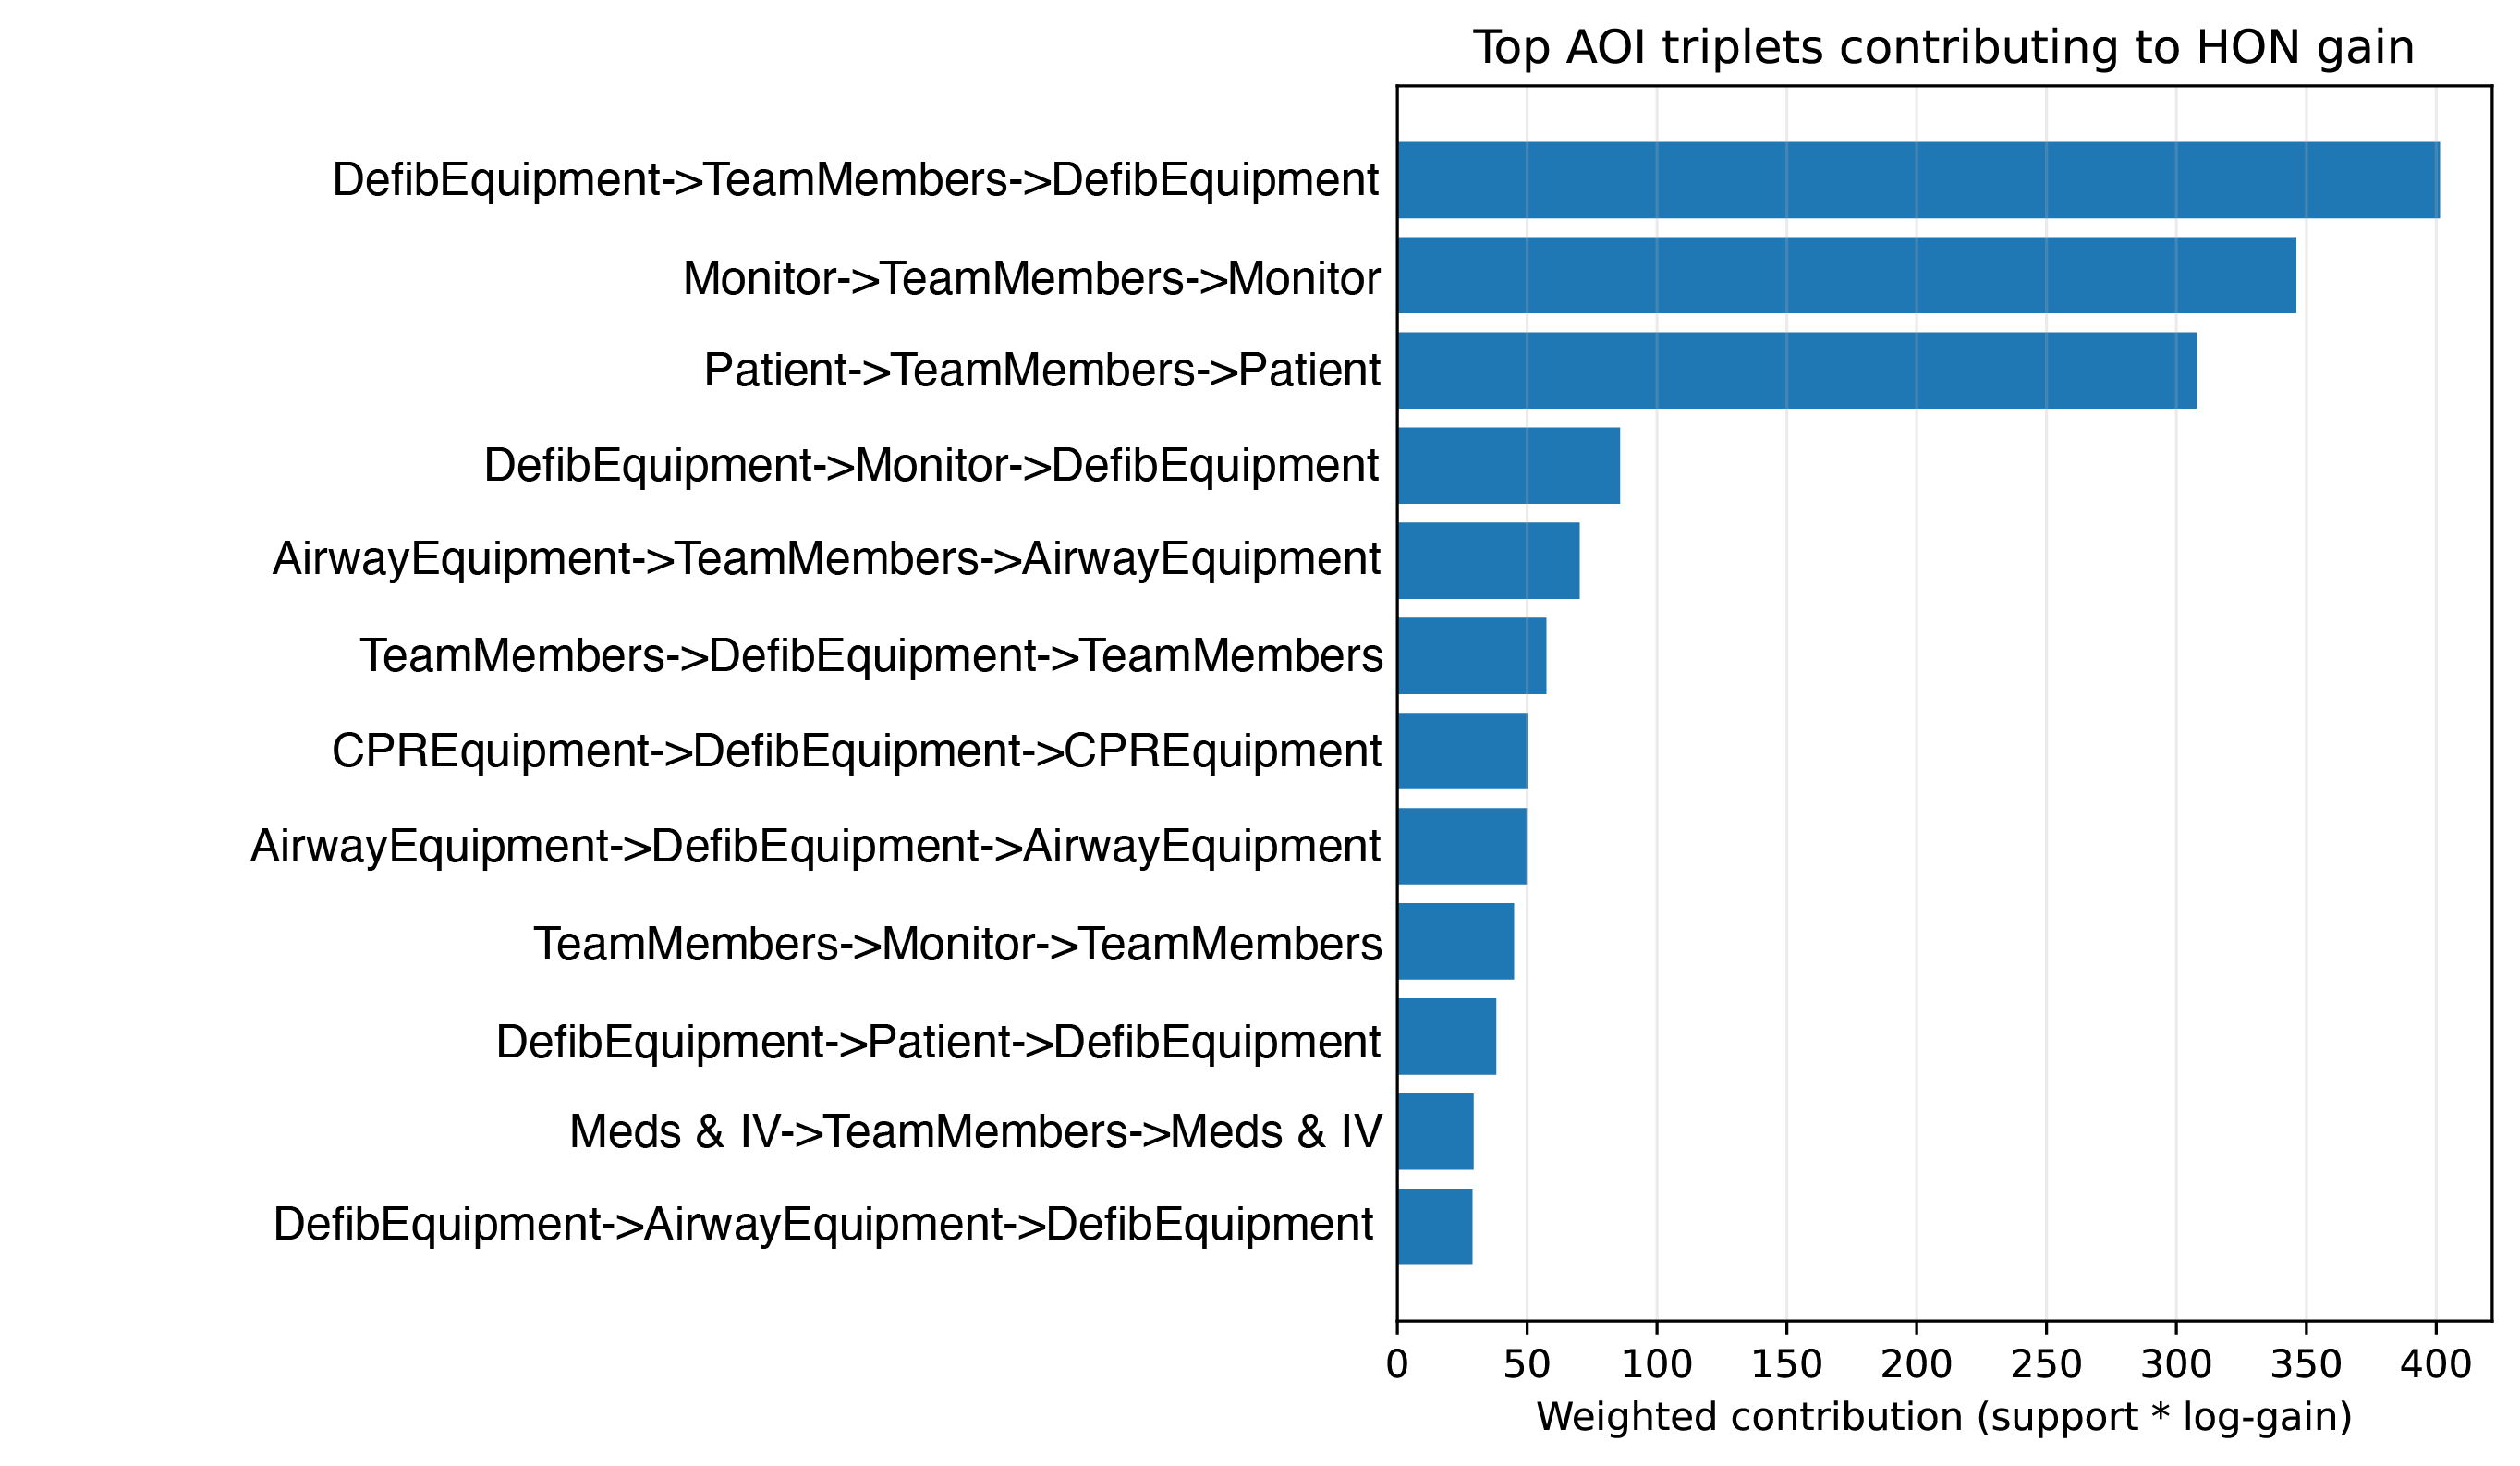
\includegraphics[width=\textwidth]{aoi_motif_top_weighted_contribution.png}
\caption{Top higher-order motifs (length-2 contexts) ranked by weighted contribution to the held-out log-likelihood gain of HON($k{=}2$) over first-order. Most are short return-to-anchor triplets ($A{\to}B{\to}A$) involving \textit{Equipment\,--\,Defib}, \textit{Patient Vitals Monitor}, and \textit{Patient}, indicating structured monitoring loops.}
\label{fig:motifs}
\vspace{-6pt}
\end{figure}

To localize \emph{where} the AOI-only gain originates, we ranked length-2 contexts by their weighted contribution to the LOSO log-likelihood difference between HON($k{=}2$) and first-order (Fig.~\ref{fig:motifs}). The dominant contributors share a \emph{return-to-anchor} shape $A \rightarrow B \rightarrow A$, in which the TeamLead briefly looks away from a focal AOI ($A$) to consult an adjacent AOI ($B$) and then returns. The strongest routines involve \textit{Equipment\,--\,Defib}, \textit{Patient Vitals Monitor}, and \textit{Patient} as anchors, with monitor and patient typically serving as $B$. A first-order model cannot represent these triplets: from state $B$ it must commit to a single outgoing distribution regardless of which AOI was visited two steps ago. The $k{=}2$ model resolves exactly this ambiguity, which explains why the macro-F$_1$ gain exceeds the accuracy gain: return-to-anchor structure reroutes probability mass toward the historically correct $A$ and away from the marginal-mode prediction.

Behaviorally, these sequences are consistent with a leader's monitoring rhythm: brief consultative glances away from a primary referent (the defibrillator during a shock cycle or the patient during a pulse check) followed by an active return to verify the consequence of an action, consistent with supervisory monitoring as cyclic verification rather than open-ended exploration~\cite{rosenman2016assessing,nallamothu2018resuscitation}. Methodologically, this clarifies the scope of first-order TNA: descriptive role and stage contrasts remain valid as summaries, but the \emph{generative} mechanism producing them operates over short windows of AOI history rather than single transitions.

\subsection{Limitations \& Future Work}

Our proof-of-concept study has several limitations. First, the dataset is limited to the TeamLead role and a single VR-based STEMI scenario, so generalization to other roles, scenarios, and real settings remains to be tested~\cite{kolbe2019laborious}. Second, with seven AOIs and 14 sessions, $k{=}3$ contexts are systematically under-supported, constraining the order search to short histories. Third, the stage-conditioned variant uses fixed annotations; we do not yet test data-driven change-point or soft-mixture alternatives. Finally, the smoothing strength ($\alpha{=}0.5$) was fixed a priori rather than tuned, and a sensitivity analysis is left to future work. We also selected the order $k$ and evaluated it on the same LOSO folds; the effect is large, and its bootstrap intervals are well clear of zero, but fully nested cross-validation would remove any residual model-selection optimism.

Building on these findings, a key next step is to establish the educational and clinical value of the identified return-to-anchor ($A\rightarrow B\rightarrow A$) patterns with clinicians and medical educators. For example, by having them judge whether these monitoring behaviors distinguish effective from ineffective situational awareness or expert from novice team leadership in simulation. This could inform post-simulation debriefing visualizations that surface a leader's monitoring behaviors, guide attention-based training feedback, and, ultimately, provide real-time indicators of degraded situational awareness during patient care, due to e.g., high cognitive load. Methodologically, the approach should also extend beyond the TeamLead role and the single cardiac arrest scenario, incorporate deeper histories as larger corpora permit, compare soft or change-point stage encodings against hard partitions, and integrate gaze with communication and action streams for joint models of team coordination.

\section{Conclusion}

We showed that a second-order Markov model is a promising and parsimonious approach to modeling team lead gaze in clinical simulation. Unlike a first-order model, it enables capturing recurring sequential visual attention structures, e.g., monitoring cycles such as monitor → patient → monitor — and outperforms the first-order baseline across all evaluation metrics. 


existing computation methods novel setting noise data and able to derive clinical educational meaningful findings,  test, extended future work. if it is apply to different.........
 approach is a contribution new application using HON in gaze at dynamic acute care setting for educational and clinical findings. overfixating->monitoring behavior from data level, clinical-> clinical management, why somebody in diagnostic gaps, lacking knowledge, misrecoginize heart rthym. educational->

\bibliographystyle{splncs04}
\bibliography{mTEAM_HON}

\end{document}
